% Chapter 12 -- translated by Claude (2026), continuing the voice and
% register of the Burkett-Hutcheson chapters.

\chapter{Tools for graphing}

\section{Introduction}

Your calculator has powerful graphing capabilities. In turn,
Symbulator includes two useful tools for graphing: one for Bode
diagrams and one for functions of time $t$.

\section{The bode tool}

The \code{bode} tool allows making Bode diagrams. It is executed
like this:

\begin{entry}
sq\bode()
\end{entry}

It is very easy to use. Let us learn to use this tool by solving a
real problem. We will use one that Professor Edilberto Yee, of the
Technological University of Panama, gave us as the final homework of
the Electronics III course.

\problem{087}

\emph{Problem: Make the Bode gain diagram for $V_o/V_g$, from
$10^{4}$ to $10^{13}$~rad/s, for the following circuit.}


% figures added 10 Sep 2026
\begin{figure}[!ht]
\centering
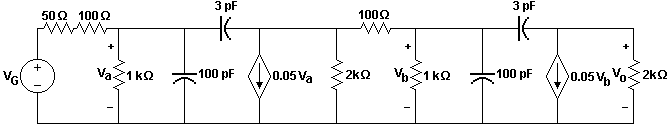
\includegraphics[width=150mm]{book_figures/p087_0.png}
\caption*{Circuit for Problem 087}
\end{figure}

% figures added 10 Sep 2026
\begin{figure}[!ht]
\centering
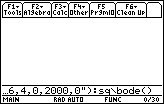
\includegraphics[width=56mm]{book_figures/p087_1.png}
\caption*{The command for Problem 087, on the TI-89}
\end{figure}

Solution: As we have already explained, when dealing with large
circuits, a simulation with exact values will give us precise
answers, while a simulation with approximate values will give us
fast answers. Since this problem was homework to solve at home, time
was not critical, and we preferred to use exact values, to assure
the precision of the answers.

We give the command to run the simulation in the frequency domain,
and immediately after order the execution of the \code{bode} tool:

\begin{entry}
sq\fd("e1,5,0,vg,0;r1,5,1,150,0;r2,1,0,1000,0;
      cc1,1,0,10^-10,0;cc2,1,2,3*10^-12,0;jd1,2,0,5/100*v1,0;
      r3,2,0,2000,0;r4,2,3,100,0;r5,3,0,1000,0;
      cc3,3,0,10^-10,0;cc4,3,4,3*10^-12,0;jd2,4,0,5/100*v3,0;
      r6,4,0,2000,0"):sq\bode()
\end{entry}

We press \key{ENTER}. The simulation takes around 3 minutes. At the
end, the \code{bode} tool executes. The tool presents us a small
menu, which asks us to choose between making a Bode plot or cleaning
up the variables created.

We choose the first option of this menu. The second is used when,
after having made some graphs, we wish to finish the work and clean
up the variables the tool has created. So, we select Bode Plot and
press \key{ENTER}. A menu appears. In this menu we must enter the
following:

\emph{Transfer function.} Here we place the transfer function whose
graph we wish to make. We can write the function itself, or place
the names of the variables that define it. In our case, we place
\code{v4/v5}, that is, $V_o/V_g$.

\emph{Independent variable.} It is the variable that represents the
frequency. It is almost always \code{s}. We place \code{s}.

\emph{Type of diagram.} There are three types: gain (Gain Plot),
phase (Phase Plot) and both (Both Plots). If gain or phase is
chosen, the complete screen will show the graph. If both is chosen,
the screen will divide in two to show gain above and phase below. In
our case, we select Gain Plot. To return the screen to its original
form afterwards, go to \key{MODE} and set the Split Screen mode to
FULL.

\emph{Minimum frequency.} It must be greater than zero. In our case,
we place \code{1E4}.

\emph{Maximum frequency.} It must be greater than the minimum. In
our case, we place \code{1E13}.

\emph{Units of the frequency.} It serves to specify in what units we
entered the frequencies above. In our case, we select rad/sec.

We press \key{ENTER}. A message appears, announcing that the units
of the vertical axis are decibels (dB), and those of the horizontal
axis are the logarithm of the frequency in radians/second.

We press \key{ENTER}. After about a minute, the diagram appears.

This graph is the correct one. Obtaining it allowed me to receive
full marks on the assigned homework. Having obtained it with a
simulator made by myself, made me in addition worthy of the respect
of Professor Yee, whom I hold in very high esteem.

Here the homework ends. However, suppose we had also been asked for
the phase diagram. There is no need to run the simulation again,
because the variables \code{v4} and \code{v5} are still in memory.
It is enough to run the \code{bode} tool again:

\begin{entry}
sq\bode()
\end{entry}

The previously entered values are still there. This is thanks to
certain variables the tool generates, which can be deleted at the
end. We leave everything the same, but select Phase Plot.

We press \key{ENTER}. A message appears, announcing that the units
of the vertical axis are radians, and those of the horizontal axis
are the logarithm of the frequency in radians/second.

We press \key{ENTER}. After about a minute, the diagram appears.

Having finished, we run the tool again and choose Clean \& Exit to
clean up the created variables.

\section{The plot tool}

The \code{plot} tool allows graphing functions of time $t$. It is
executed like this:

\begin{entry}
sq\plot()
\end{entry}

It is also very easy to use. Let us learn to use this tool by
solving a real problem. We will use a problem that Professor Eliane
Boulet de Cabrera, of the Technological University of Panama,
presented to her students in an examination. In that examination the
graph of the answers was not requested, but we can use it to
illustrate the use of the tool.

\problem{088}

\emph{Problem: Given the following circuit, find the complete
response for $v_2(t)$ and $v_1(t)$ for $t > 0$. Then, graph the
value of $v_2(t)$ and $v_1(t)$ vs time, from 0 to 7 seconds.}


% figures added 10 Sep 2026
\begin{figure}[!ht]
\centering
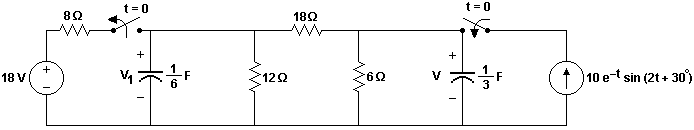
\includegraphics[width=150mm]{book_figures/p088_0.png}
\caption*{Circuit for Problem 088}
\end{figure}

Solution: We will use exact values for precision, but we will save
time using FD instead of TR, because in the middle of an examination
time is very valuable. We give the command to run the simulation in
direct current, to find the initial conditions:

\begin{entry}
sq\dc("e1,3,0,18;r1,3,1,8;cc1,1,0,1/6;r2,1,0,12;r3,1,2,18;
      r4,2,0,6;cc2,2,0,1/3")
\end{entry}

For \code{vcc1} we obtain 9. For \code{vcc2} we obtain 9/4. These
will be our initial conditions for the next interval. We give the
command to run the simulation in the frequency domain:

\begin{entry}
sq\fd("cc1,1,0,1/6,9;r2,1,0,12,0;r3,1,2,18,0;r4,2,0,6,0;
      cc2,2,0,1/3,9/4;js,0,2,10*e^(-t)*sin(2t+30°),0")
\end{entry}

We press \key{ENTER}. The simulation executes, with the
participation of the (Impala) Mode. Now we are going to obtain the
answers, and at the same time we will store them in variables, to be
able to invoke them later from the \code{plot} tool. We use
\code{sq\char`\\fd\_to\_tr(v1)}. We obtain a very voluminous
symbolic expression. For that reason, we use
\code{expand(approx(ans(1)),t)→v1t} and obtain the complete answer
in approximate form for the voltage in the capacitor on the left:

\begin{entry}
-.667*e^(-t)*cos(2.*t)-2.33*e^(-t)*sin(2.*t)
   +13.8*e^(-t/2)-4.16*e^(-t)
\end{entry}

With \code{expand(approx(sq\char`\\fd\_to\_tr(v2)),t)→v2t} we obtain
the complete approximate answer for the voltage in the capacitor on
the right:

\begin{entry}
-13.7*e^(-t)*cos(2.*t)+5.17*e^(-t)*sin(2.*t)
   +13.8*e^(-t/2)+2.08*e^(-t)
\end{entry}

Now we can execute the \code{plot} tool:

\begin{entry}
sq\plot()
\end{entry}

A menu appears, in which we must insert three data:

\emph{Function.} It is the function of time $t$ we wish to graph. In
our case, \code{v2t}. This is the name we gave the variable in which
we stored the voltage in the time domain.

\emph{Minimum time.} It is the minimum time of the graph, that is,
the left end of the horizontal axis. In our case, 0.

\emph{Maximum time.} It is the maximum time of the graph, that is,
the right end of the horizontal axis. It must be greater than the
minimum. In our case, 7.

We press \key{ENTER}. The graph appears.

Once we have this graph ready on the screen, we can apply over it
all the graphing commands the calculator has. For example, the
maximum value command. For more information on these commands,
consult the User's Manual.

To obtain the graph of the voltage $v_1$, the same procedure is
repeated, but entering \code{v1t} as the function to be graphed.

With this, we have finished the problem. As was to be expected, the
\code{plot} tool can also graph functions that are not Symbulator
answers. For example, if we enter as the function the following:
$e^{-t}\sin(10t)$, and graph between 0 and 3 seconds, we will obtain
its graph.

In this way, we have finished this book about the Symbulator.
